- German guidelines for traffic signals (Richtlinien für Lichtsignalanlagen (RiLSA))

- Different traffic light sensors (accuracy, features, can they measure the number of vehicles?, how is the data accessible?, how widely used are ones that are accessible over the internet currently?)

- Neural networks, but details on that have to be read up first (The general idea must be explained in the introduction really well. Why did we choose neural networks?)

- Maybe some statistical data analysis method for defining the optimal stress levels to switch signals and stress level growth?

- Open Street Maps (what data can they carry? can we use them for our endeavor?)

-> Should we introduce all these topics when they are important? Maybe have just some basic stuff here like german guidelines, traffic light sensors and neural networks? The choice of Open Street Maps may need to be explained in more detail.

\newpage

\section{Artificial Neural Networks}

Artificial neural networks (ANNs) is an important field in machine learning and cognitive science. There are many different kinds of ANNs, but all have in common that they are inspired by biological neural networks like the human brain. The big advantage of neural networks is that neural networks can learn behavior like classification from a set of example data and do not have to explicitly modeled. ANNs are typically a set of interconnected neurons. Figure \ref{neuron} shows the structure of a neuron.

\begin{figure}[ht]
	\centering
  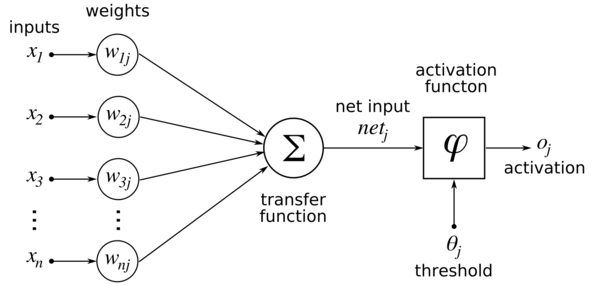
\includegraphics[scale=0.6]{figures/neuron_structure.png}
	\caption[Structure of a neuron]{Structure of a neuron \protect\footnotemark}
	\label{neuron}
\end{figure}
% https://upload.wikimedia.org/wikipedia/commons/thumb/6/60/ArtificialNeuronModel_english.png/600px-ArtificialNeuronModel_english.png
\footnotetext{wikipedia}

A neuron has a set of $n$ input variables $x_1, x_2, x_3, ..., x_n$ which either are the output of another neuron or the input to the neural network that is given by the user. Each input variable is multiplied with a weight $w_1j, w_2j, w_3j, ..., w_nj$ where $j$ is the iteration of the weight. All of the products of the variable and its specific weight are then summed and passed to an activation function that determines what the result is. Examples for the activation function would be a step function that just compares the value to a threshold and puts out 0 or 1 or a sigmoid function that puts out a value between 0 and 1. The output can then be given to the connected neurons or the output of the neural network.

Somehow get from neurons to different types of neural networks.

There are multiple different types of ANNs. They are divided by the form of learning. This depends on how the learning set given to the neural network is created and composed. With supervised the learning set consists of pairs of input and output vectors and it thrives to adjust the weights of the neural network so that it maps the function described by the learning set. Then there is unsupervised learning which just takes for example a cost function, that calculates some costs from the input and output of the ANN, and a learning set, only consisting of data, and tries to minimize the cost function by adjusting the weights. The third possible scenario is reinforcement learning. This happens when there is no data set to learn from, but an agent interacts with some world and learns what interactions are good and what are bad by observing the effects. This is for example used when an artificial intelligence that plays chess is playing against itself to get better.

Another important aspect of ANNs is how the neurons are interconnected. The most basic structure of ANNs are feedforward neural networks. In this model the neural network is divided into layers and every layer only passes its information to the next layer. In contrast to that there are recurrent neural networks that allows the graph of neurons to have cycles. This allows the network to have some kind of memory and keep values to use in later iterations. An example for the use of recurrent neural networks would be a word processor that takes single words but can process whole sentences by memorizing what words were already passed through. There are a lot of sub categories of these structures and other architectures of ANNs, but these are the most important and the ones relevant for this thesis.

Feedforward neural networks that only have an input layer and an output layer are called perceptrons. They are the simplest kind of neural network, but they are very limited in their use. === Linear separability / XOR === The advantage of this kind of neural network is that it does not need a lot of learning data and can use a really simple learning algorithm called the delta rule.

=== Maybe a perceptron is enough for the prediction? ===

=== delta rule ===

A bit more complex than perceptrons are multilayer perceptrons. They not only have an input and an ouput layer, but also one to several hidden layers that get fed from the previous layer and feed into the following layer. With this architecture more complex problems like XOR can be solved. The structure and weights of an XOR neural network are shown in figure \ref{multilayer_XOR}

\begin{figure}[ht]
	\centering
  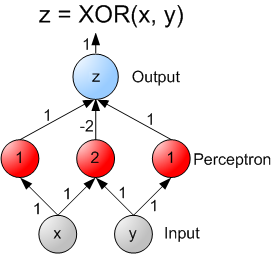
\includegraphics[scale=1]{figures/multilayer_XOR.png}
	\caption[Structure of multilayer perceptron that implements an XOR]{Structure of multilayer perceptron that implements an XOR \protect\footnotemark}
	\label{multilayer_XOR}
\end{figure}
% https://upload.wikimedia.org/wikipedia/commons/7/7b/XOR_perceptron_net.png
\footnotetext{wikipedia}

The more complex the network and input and output the more data has to be learned from.